\documentclass[journal]{Imperial_lab_report}

\usepackage[utf8]{inputenc}
\usepackage{graphicx}
\usepackage{cite}
\usepackage{amsmath}
\usepackage{url}
\usepackage{float}
\usepackage{bm}
\usepackage{hyperref}
\usepackage{physics}
\usepackage{listings}
\usepackage{xcolor}
\usepackage{siunitx}
\usepackage{ragged2e}
\usepackage{url}
\usepackage[siunitx, european, cuteinductors]{circuitikz}
\usepackage{circuitikz}
\usepackage{subfig}
\usepackage{tabularray}
\renewcommand{\thetable}{\arabic{table}}
\renewcommand{\thefigure}{\arabic{figure}}
\usepackage{comment}
\usepackage{gensymb}
\usepackage{xmpmulti}
\usepackage[british]{babel}
\usepackage{hhline}
\usepackage{multirow}


\hypersetup{
  colorlinks=true,
  linkcolor=black,
  filecolor=black,   
  urlcolor=black,
  citecolor=black
}


\newcommand{\midlabelline}[3]{
   \node (midlabel) at ($ (#1)!.5!(#2) $) {#3};
   \draw[latex-] (#1) --  (midlabel);
   \draw[-latex] (midlabel) -- (#2);
}


\begin{document}
\title{Correcting the Mercury Emission Spectrum for the Irregular Motion of a Stepper Motor}


\author{Maanas Kishorekumar Bysani}% <-this % stops a space




% The paper headers
\markboth{Maanas K Bysani}
{Shell \MakeLowercase{\textit{et al.}}:}


% make the title area
\maketitle

% As a general rule, do not put math, special symbols or citations
% in the abstract or keywords.

\begin{abstract}
In this report, our primary aim was to obtain Mercury's emission spectrum using a Michelson Interferometer and a Mercury-vapor discharge lamp, and correct the obtained interferogram for the irregular motion of the motor, using Mercury's green line at 546.07 nm as a reference. We make use of Fourier theory to arrive at the spectral decomposition by Fourier Transforming the interferogram. Five well-defined peaks corresponding to the five distinct 'strong' wavelengths in the visible region were obtained: 404.62 nm, 435.79 nm, 546.03 nm, 576.92 nm, and 579.03 nm with a low uncertainty of 0.20 nm, making them fall within the tolerance of the literature values.
\end{abstract}
\vspace{-12pt}


\section{Introduction}
\IEEEPARstart{I}{n} this experiment we made extensive use of spectroscopy techniques to analyse the absorption spectrum of naturally abundant Rubidium. We obtain the fine \textbf{(FS)} and hyperfine \textbf{(HFS)} structure splitting through Doppler-broadened \textbf{(DB)} and Doppler-free \textbf{(DF)} spectroscopy which provides a coarse calibration of wavelength to timebase of the oscilloscope. We then use a (confocal) Fabry-Perot interferometer (FP) to better this calibration by analysing the resultant interference modes which are sensitive to nanometer-scale [check] changes in wavelength, making it incredibly accurate. The Fabry-Perot interferometer is a critical component of most complex optical setups with a tunable laser, given its applicability to laser-locking and frequency stabilisation. The FP holds significant value as it helped prove the quantum theory, and in more recent times has applications in several areas of physics including gravitational wave detectors where it is used to \textit{store} photons for milliseconds and CQED where it has been used to establish ultra-high finesse ($4*10^9$) resonators. [cite][change wording]

\vspace{-5pt}

\section{Background}
\IEEEPARstart{T}{he} MI has a simple structure made up of a light source, a beamsplitter and two mirrors which reflect each of the split beams. These reflected beams interfere constructively or destructively based on whether their relative Path Difference (PD) is an integral multiple of their wavelength or not, resulting in a pattern of fringes that can be measured. Constructive interference occurs when $PD = m\lambda$ and destructive interference occurs when $PD = (m+\frac{1}{2})\lambda$. Varying the PD by a fraction of the wavelength will change the pattern observed, making the MI an incredibly precise ruler. Figure \ref{fig:setup} shows the setup we used for our experiment: the Linear Translation Stage Mirror (M1) can be moved towards/away from the beamsplitter using a motor-driven screw gauge, and the Kinetic Mirror (M2) was clamped at an equal distance from the beamsplitter and adjusted only its tilt angle during the experiment. The MI was said to be aligned when a single fringe using a standard laser was observed, and as figure \ref{fig:alignment} shows, this was the point where both the mirrors were parallel.

%(along with a compensating plate for correction, if needed)
\begin{figure}[h]
\centering
\captionsetup{font=footnotesize}
    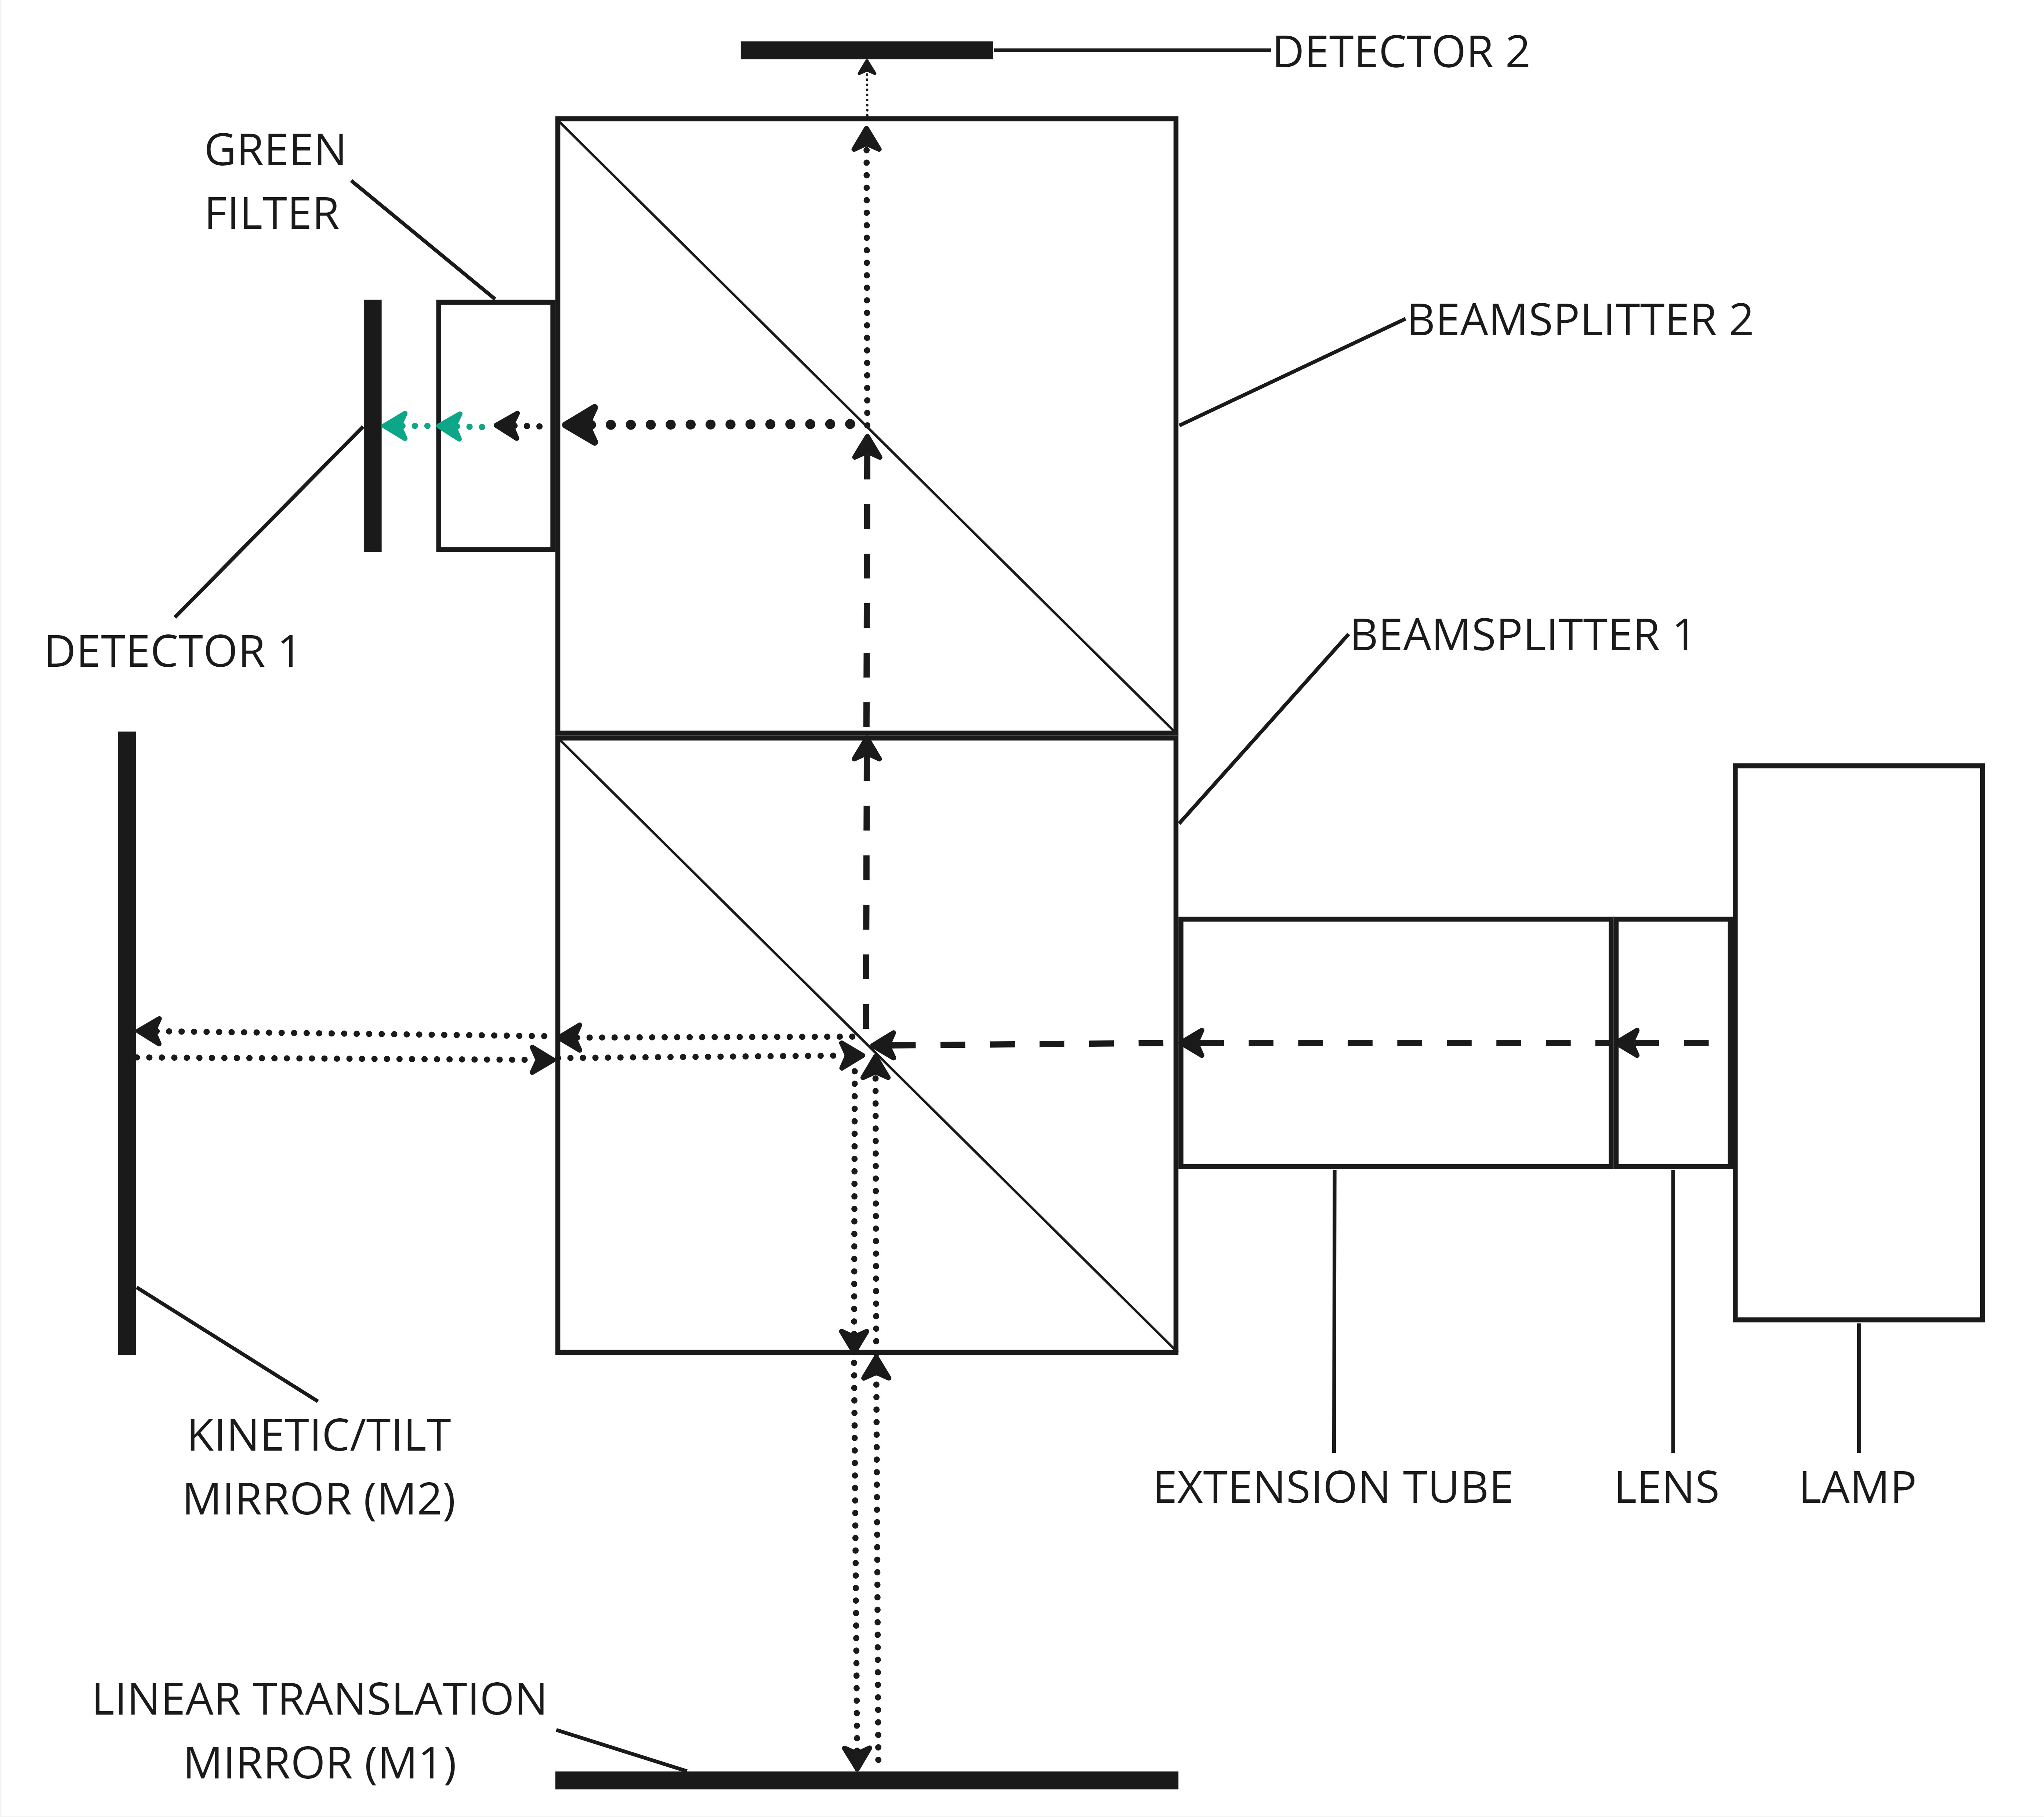
\includegraphics[width = 0.5\textwidth]{setup.jpg}
    \caption{Our final setup with which we collected two sets of data simultaneously to correct the Mercury spectrum using its well-defined green line.}
    \label{fig:setup}
\vspace{-15pt}
\end{figure}

\begin{figure}[h]
\centering
\captionsetup{font=footnotesize}
    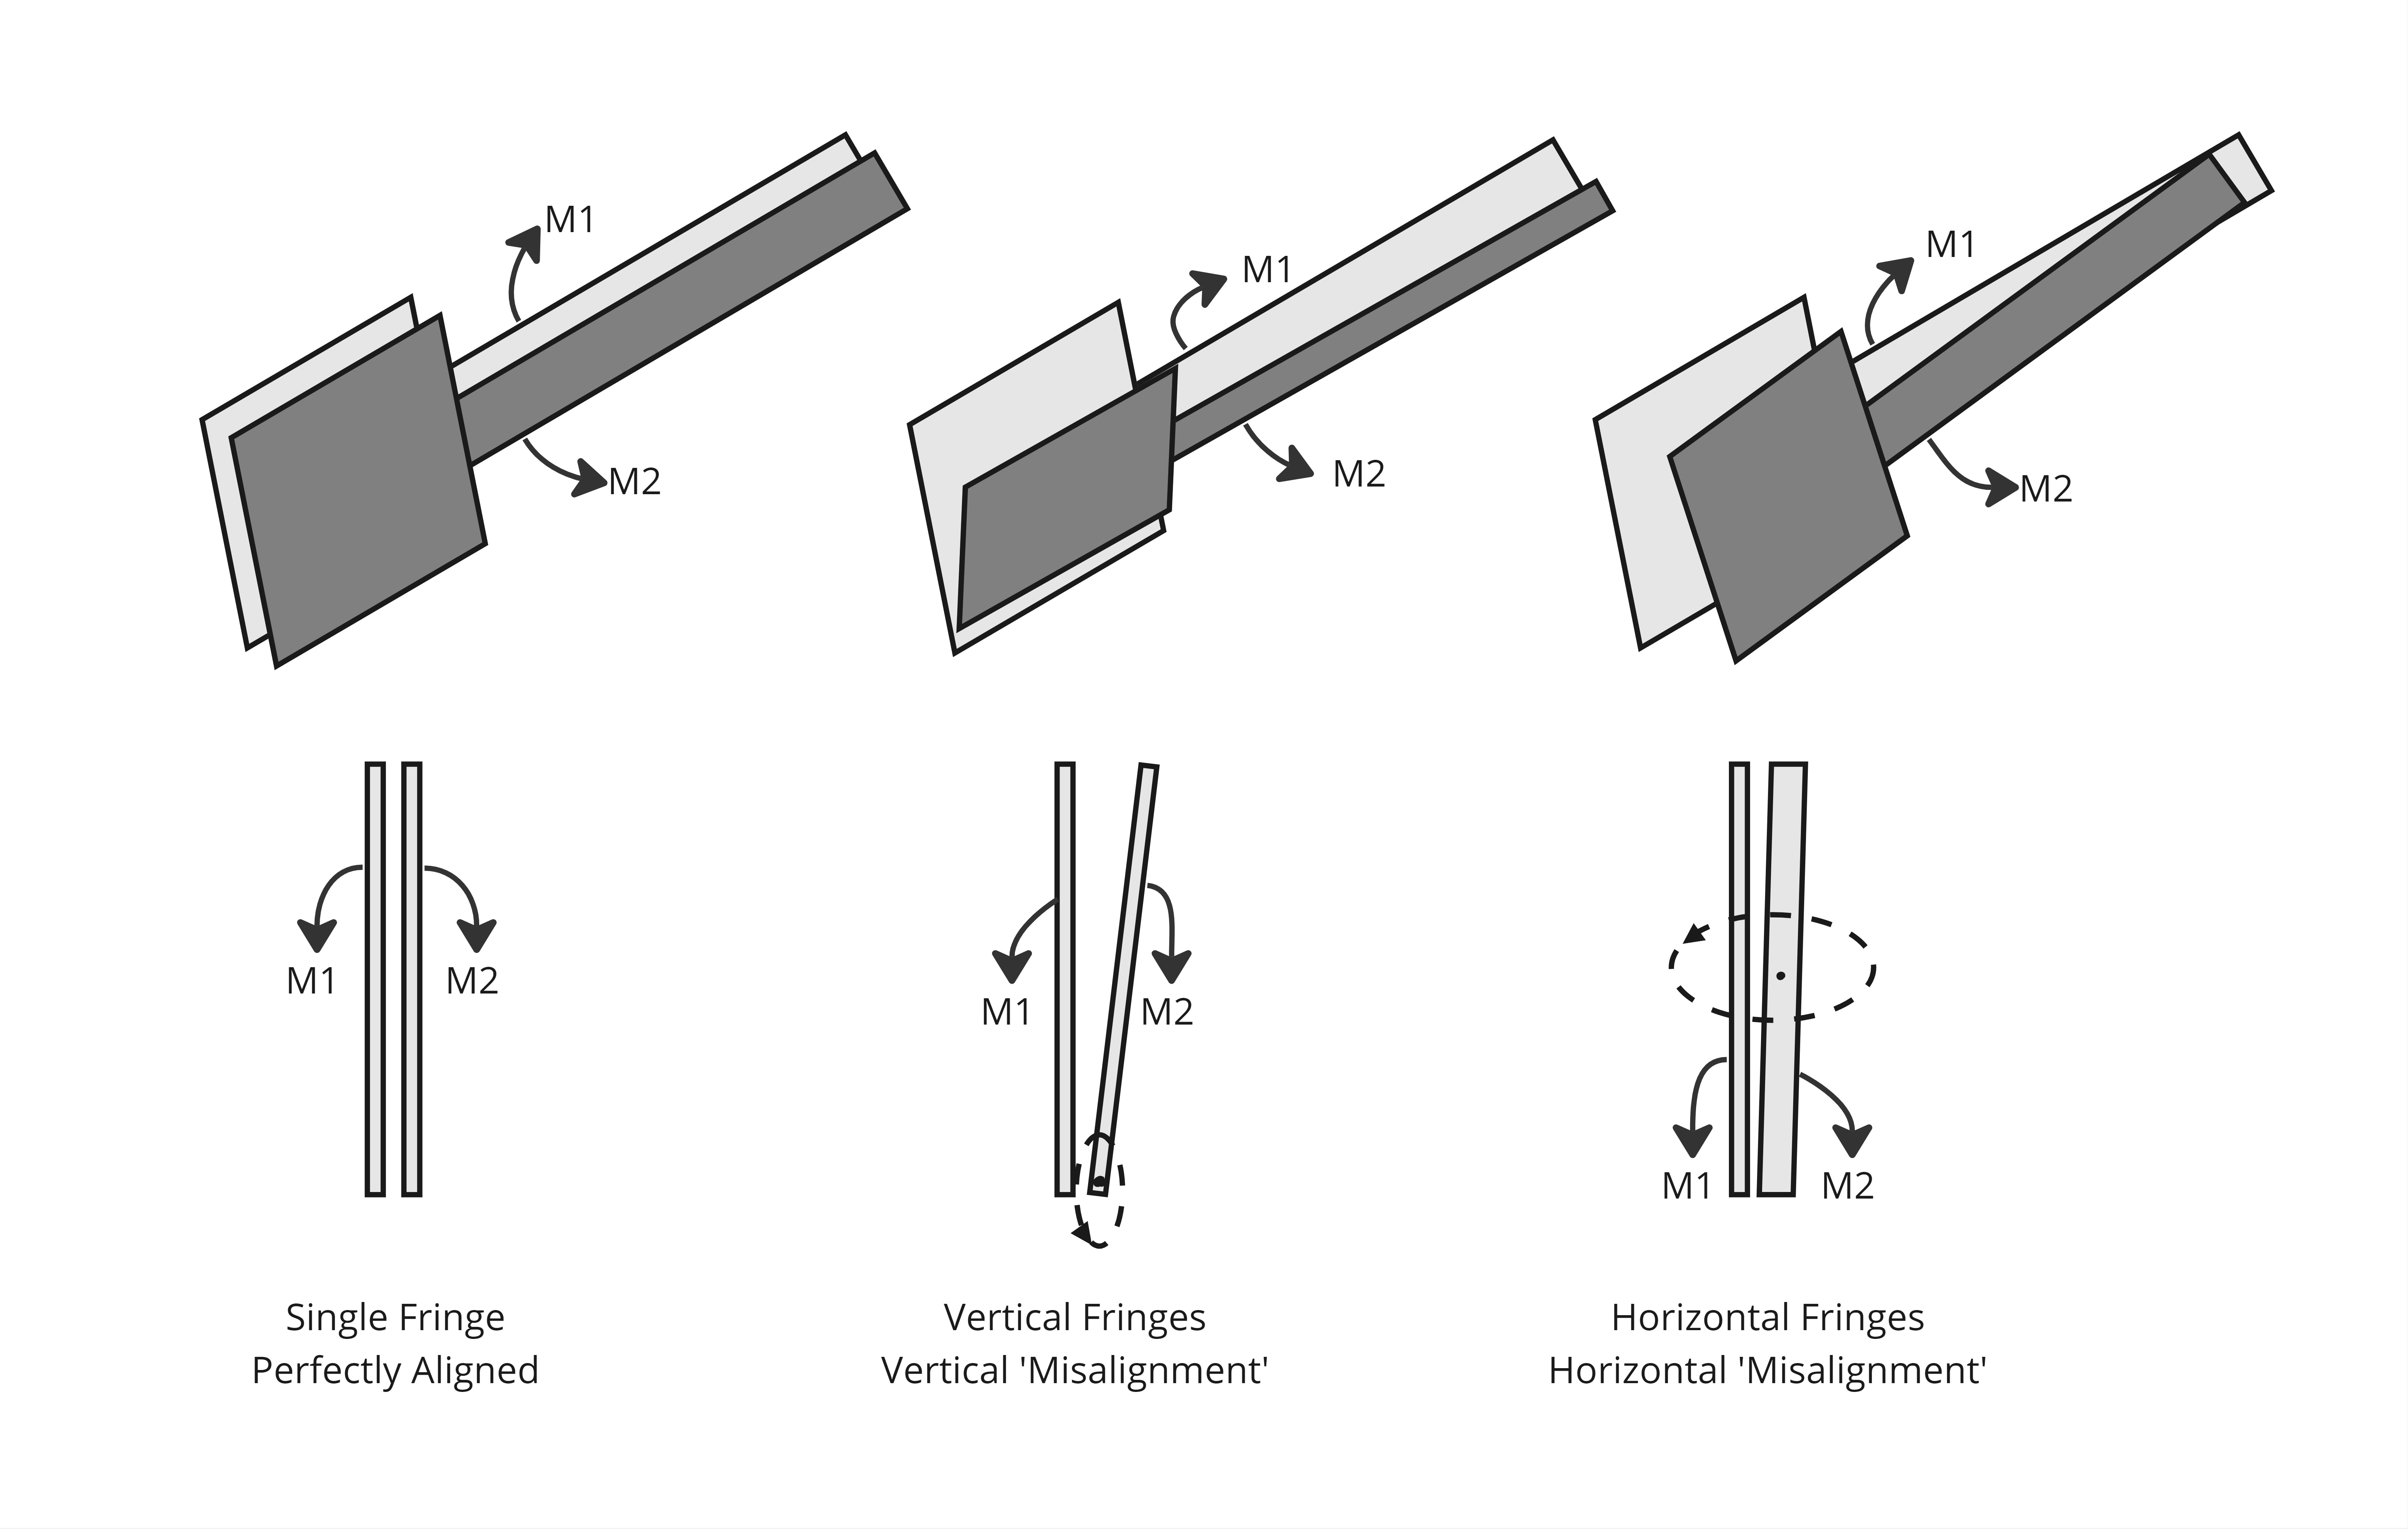
\includegraphics[width = 0.5\textwidth]{alignment.png}
    \caption{The different tilt settings of M2 and the resulting orientation of the straight line Fizeau fringe patterns observed using a standard laser.}
    \label{fig:alignment}
\vspace{-20pt}
\end{figure}

We can see the merits of this method when we analyse a source made up of multiple wavelengths. We obtain a complicated-looking interferogram as there are multiple combinations of PDs for which we obtain a constructive/destructive fringe pattern. However, we know that the resulting pattern is essentially a mathematical combination of the different individual patterns. So, it is possible to decompose the complex interferogram to obtain the individual wavelengths; there are multiple methods to do this, but we will continue by (computationally) Fourier Transforming the interferogram.

Each of the spectral lines emitted by most spectral lamps has an approximately Gaussian intensity profile due to broadening effects, some originating from the quantum mechanical description of atoms itself and some from the randomness caused by neighbouring particles \cite{line_spectra_shape}. We know that a Gaussian's Fourier Transform is also a Gaussian with a standard deviation equal to the reciprocal of the original Gaussian's standard deviation. This implies that we should expect our interferogram to have a Gaussian profile, and for many-wavelength sources, a set of (convolution) Gaussian profiles.


The relationship between the width of the spectrum $\Delta f$ to the coherence length $L$ is given by \cite{coh_length_eq1}\cite{lab_manual}:
\begin{equation}
    \Delta f \cross L = \frac{c}{2\pi}, \label{eqn: width relation frequeny}
\end{equation}
where $c$ is the speed of light. The entire argument above is equally valid when we use the wavelength-wavenumber domains; following a few simple conversions of terms, we get the equivalent of equation \eqref{eqn: width relation frequeny} to be ]\cite{lab_manual}:
\begin{equation}
    \Delta\lambda = \frac{\lambda^2}{2\pi L}. \label{eqn: width relation wavelength}
\end{equation}

By inspecting the above equations we see that a source with a large $L$ ($\sigma$ of interferogram) results in a spectrum with a small $\Delta\lambda$ ($\sigma$ of spectral line), and vice versa which is consistent with the Fourier theory discussed above.



The Mercury vapour lamp works just as any gas discharge lamp \cite{Mercury_lamp_workings}: atoms are first excited to different states by an electric current flowing through the discharge tube, and the atoms then emit radiation when they de-excite and return to their ground state. The photons emitted have energies equal to the difference between the atom's energy levels, and hence each element has a characteristic emission spectrum; we use Mercury's characteristic emission spectrum \cite{Mercury_spectrum} to verify our results. The only difference is that Mercury lamps contain liquid Mercury which requires a non-zero amount of time to vaporize and ionise, hence we allowed the lamp to reach maximum intensity before collecting data. The tube also contains small amounts of argon gas which is used to start the Mercury-vaporisation process.

To correct the spectrum for the irregular movements (due to external factors such as footsteps and internal factors such as mechanical delays) of the linear translation stage motor (thus M1), it is common practice to use a known wavelength as a reference and fit (expand/shrink) the original interferogram accordingly. Once we adjust the fitted interferogram to ensure that the points are evenly distributed, we can perform the Fourier Transform on it to obtain the corrected (actual) spectrum of the source. We chose to use the green line of the Mercury spectrum as our reference wavelength for two reasons: it is one of the most intense spectral lines for Mercury, and it is a single line (unlike the yellow doublet) \cite{Mercury_spectrum}. As the motion is inconsistent, it is logical to take both measurements (the reference and actual) at the same time, which is why we use beamsplitter 2 to split the interfered beam; one of the outputs of beamsplitter 2 has a green filter attached while the other has no filter. 

Stepper motors are a type of brushless DC motor but its stator (the stationary part inside which the rotor is placed) is made up of several evenly spaced wire windings which act as magnets when powered and these control the start and stop position of the motor \cite{motor_diff}. Stepper motors are classified by their step angle and are often in one of two configurations: 1.8\degree or 0.9\degree which respectively correspond to 200 steps/revolution and 400 steps/revolution. It is also possible to split each step into smaller steps (microsteps) using a microstepper, allowing us to move the motor in smaller steps (typically upto 256microsteps/step) \cite{microstepping}. Mechanically, a stepper motor is similar to a spring-mass system: when moving from one position to another, the rotor doesn't immediately find the exact stop position, it actually overshoots slightly and oscillates around the stop position until it reaches the exact stop position \cite{microsteppers_mech_rel}. And, similar to the spring-mass system, the larger the distance from one position to another, the larger the oscillations.
\vspace{-5pt}



\section{Experimental Method}
\IEEEPARstart{W}{e} setup the MI as shown in figure \ref{fig:setup}. To calibrate/align the MI, we used a monochromatic Green Laser with only beamsplitter 1. The MI was said to be aligned when the distance between each of the mirrors to the beamsplitter was equal and when the spots from M1 and M2 overlapped and we could see fringes; we adjusted M2's tilt such that horizontal fringes were visible - this was an arbitrary choice we made as a way to maintain consistency throughout the experiment. For more precise alignment, we occasionally used a white LED, as it has a much smaller coherence length than the Green Laser, to find the null point - this was the position where a multi-coloured concentric interference pattern with strong contrast was observed. However, when we collected long interferograms (when M1's displacement was over 3mm), we would scan through the null point, hence there was no benefit of locating the null point precisely; however, it was crucial to verify the MI was aligned before every scan.

The entire setup shown in figure \ref{fig:setup} was made on an optical table (supported by optical table supports) which was covered on all sides with opaque sheets of black acrylic. This not only prevented leakage from the box but also ensured no stray ambient light rays entered the box. As the intensity of the Mercury lamp was relatively low compared to the other light sources, we made our entire setup more 'compact' by moving the components closer. This included placing the detectors adjacent to the outputs of beamsplitter 2 - this is allowed as the interference takes place 'inside' beamsplitter 1 as opposed to image formation using lenses (where the screen must be placed at a certain distance to observe the image). We used a 25.4mm lens with an extension tube to collimate and expand the input Mercury beam as a means to increase its intensity.


M2 had knobs to adjust its tilt; each revolution results in a tilt of approximately 8mrad \cite{tilt_settings} but since we were fixing the tilt during alignment and not changing it throughout the experiment, we can disregard the numerical level of tilt but must ensure that it stays the same throughout the experiment. M1 was connected to a lever which was itself connected to a micrometer screw gauge shaft driven by a stepper motor connected to a gearbox. The stepper motor itself has a 1.8\degree step angle corresponding to 200 steps/revolution, but the setup also included a micro-stepper which divides each step into 256 microsteps; resulting in a total of 51200 microsteps per revolution. Accounting for the relevant reduction ratios of this system, we determined that each microstep corresponds to a movement of 15.6 pm of M1; and in this experiment, we are also testing the validity of this approximation. The detectors' sampling frequency could also be chosen between 50Hz, 200Hz and 500Hz; we decided to use 50Hz as higher frequencies would lower the photodetector's performance.

%There are also reduction ratios which have been omitted here as they depend on each setup and, hence are irrelevant.


We were also able to adjust the speed of M1's movement. The speed combined with the sampling frequency of the detector determines the effective sampling rate of the system. We chose to stick with the 50Hz sampling rate to avoid a loss in resolution and decided to alter the effective sampling rate just by adjusting the motor speed. According to the Shannon-Nyquist sampling theorem \cite{shannon_ac1}\cite{shannon1}, we can move the motor at a maximum speed of 436800 microsteps/second which would result in two samples per wavelength. Ideally, we would want to collect the maximum number of samples per wavelength but this would take a long time as we were scanning over a long range of 200 million microsteps (in line with Fourier theory of using a long domain to obtain a high-resolution Fourier Transform), hence a tradeoff was made - we chose to use a speed of 87360 microsteps/second as it provided data with a sufficient number of samples per wavelength and did not take too long to complete (we tested different speeds and this gave the best tradeoff). The importance of collecting sufficient samples per wavelength is shown in \ref{fig:resolution}. The low-resolution case is a result of having a lower number of samples per wavelength and we see how the two peaks have merged (convoluted) to become a single, wider peak. Hence it is key that a sufficient number of samples per wavelength is being collected to get a high-resolution spectrum.

\begin{figure}[h]
\centering
\captionsetup{font=footnotesize}
    \includegraphics[width = 0.5\textwidth]{resolution (2).png}
    \caption{The need to collect sufficient samples per wavelength and its effect on the spectral decomposition: the low-resolution plot is a result of using an interferogram with a lower number of samples than the high-resolution plot and we see that one of the spectral lines is lost.}
    \label{fig:resolution}
\vspace{-12pt}
\end{figure}

\vspace{-5pt}

\section{Results \& Uncertainties}
\IEEEPARstart{B}{ased} on the green line interferogram we estimated the coherence length to be about 0.53 $\pm$ 2\% mm. Using this in equation \eqref{eqn: width relation wavelength}, we get the spectral width, $\Delta\lambda$, to be 0.10 $\pm$ 2\% nm. Therefore, if we have a sufficiently high-resolution interferogram, we will be able to resolve spectral lines up to 2$\Delta\lambda$ apart so: 0.20 nm. 

\begin{figure}
\centering
\captionsetup{font=footnotesize}
    \includegraphics[width = 0.50\textwidth]{report plot2.png}
    \caption{The resulting spectrum (with zoomed-in mini-plots showing best-fit Gaussians and its mean on the x-axis) for the Mercury lamp, corrected for the irregular motor motion using the 546.07 nm green line as a reference. The errors from the Gaussian-fitting algorithm are much smaller than the 0.20nm uncertainty defined earlier and hence have been omitted.}
    \label{fig:spectrum}
\vspace{-14pt}
\end{figure}

We ran the data collected through a high-pass Butterworth filter \cite{Butterworth}. This helps get rid of the edge effects (ringing/Gibb's phenomena \cite{gibbs}) that occur as a result of performing a Fourier Transform on a truncated dataset. The order of the filter was set to 2; ideally, we would want to use a filter of the highest order possible as this corresponds to a square-wave-like band-pass filter, but this would result in losing parts of the signal as we are dealing with a non-ideal dataset \cite{Butterworth2}. 


Once we corrected the interferogram data for the irregular motion of M1 using the green line wavelength as a reference, we performed a Fourier Transform and the resulting spectrum is shown in figure \ref{fig:spectrum}. The mean wavelengths obtained from the fitted Gaussians are shown in table \ref{table:results} along with the respective spectral widths which we defined to be the Full Width at Half Maximum (FWHM); the standard values are also listed for reference. We also used a calibrated grating spectrometer to obtain a reference spectrum, albeit at a lower resolution than the FTS - this is also included in table \ref{table:results}. The reproducibility of the results was verified when we repeated the experiment and achieved the same values; the uncertainty from taking the average of the two measurements would not hold physical significance and hence has been disregarded. 

As we collected both sets of data - the green line and the entire spectrum - simultaneously, the uncertainty is simply the minimum resolvable difference of wavelengths which we determined to be 0.20 nm earlier. Other sources of errors such as thermal effects and mechanical vibration exist but we have not been able to collect sufficient data to quantify them to an appropriate confidence level, unfortunately.  


% \begin{figure}[h]
% \captionsetup{font=footnotesize}
%     
\includegraphics[width = 0.5\textwidth]{test image.png}
%     \caption{interferogram}
%     \label{fig:figure1}
% \end{figure}


\begin{table}[h!]
  \captionsetup{font=footnotesize}
\begin{center}      
  \renewcommand{\arraystretch}{1.3}
  % \begin{tabular}{|p{1.05cm}|c|c|c|p{1.95cm}|p{1.06cm}|}
  \begin{tabular}{|c|c|c|c|c|c|}
    \hline
    \multirow{2}{*}{\textbf{Colour}} & \multicolumn{3}{c|}{\textbf{Wavelength, $\lambda$, (nm)}} & \multirow{2}{*}{\textbf{\shortstack{Spectral Width, \\ $\Delta\lambda$, (nm)}}} & \multirow{2}{*}{\textbf{Dev.}} \\
    % \hline
    % \textbf{Inactive Modes} & \textbf{Description}\\
    \cline{2-4}
    & \textbf{Liter.} & \textbf{GS} & \textbf{Meas.} & & \\
    %\hhline{~--}
    \hline
    Purple & 404.66 & 404.60 & 404.62 &  0.09 & -0.03 \\ \hline
    Blue & 435.83 & 435.65 & 435.79 &  0.08 & -0.04\\ \hline
    Green & 546.07 & 545.91 & 546.03 &  0.09 & -0.04\\ \hline
    Yellow I & 576.90 & 576.86 & 576.92 &  0.11 & -0.04\\ \hline
    Yellow II & 579.00 & 578.89 & 579.03 &  0.11 & -0.04\\ \hline
  \end{tabular}
\newline \caption{Values from Literature \cite{Mercury_spectrum}, the Grating Spectrometer (GS) and what we Measured along with the Deviation between the Measured and Literature values for each of the five wavelengths detected. The Grating Spectrometer and Measured Wavelengths were obtained by fitting a Gaussian and determining its mean. The spectral width is for the Measured values which corresponds to the standard deviation (FWHM) of the fitted Gaussian.}
\label{table:results}
\end{center}
\end{table}
\vspace{-10pt}


% \begin{figure}[h]
% \captionsetup{font=footnotesize}
%     
\includegraphics[width = 0.5\textwidth]{test image.png}
%     \caption{microsteps distribution}
%     \label{fig:figure1}
% \end{figure}

We also obtained the microstep:M1 ratio to be 19.1 pm which indicates a 22.2\% error with the calculated approximate value of 15.6 pm, implying that correction was necessary and plays a significant role.

\section{Discussion}
\IEEEPARstart{T}{he} MI being a highly precise and accurate system also makes it one that is extremely sensitive to several microscopic factors that are often difficult to measure and quantify. Some of these factors are discussed in this section along with ways to quantify them. 
\vspace{-10pt}

\subsection{Thermal Changes \& Mechanical Stress Relaxation:}
The motor and micrometer are held in tension while scanning to collect data and once the microcontroller's power supply is switched off, the stepper motor can no longer provide the 'holding torque' to stay at the same position it stopped at. Apart from this, as all the components were screwed to the steel breadboard using a clamping fork, thermal changes could affect its 'tightness' causing it to move out of position. While we realigned the MI at the start of every session, changes during the recording period were unaccounted for, however, the data doesn't seem to reflect any significant misalignment.
\vspace{-18pt}

\subsection{Random Undesirable Vibrations:}
During preliminary experiments, we noticed that the MI was susceptible to very small vibrations such as typing on the keyboard beside the MI, briskly walking past the setup and moving chairs and benches. During the actual experiment, my lab partner and I moved away from our setup to prevent any unfavourable 'noise' from affecting our data, however, our colleagues were still performing their experiments beside our setup and walking past it, which was out of our control. This could have had a significant contribution to the data collected. Furthermore, the optical table supports of the steel breadboard had a transmissibility ratio of $>$ 1 for frequencies around 1Hz \cite{optical_table_supports} - this is the average frequency of walking and for many other common human activities. 

To understand the effect of such noise and its significance on the data, we would need another detector which detects the ambient light, and we can then perform a simple subtraction to extract the noise-free signal which we can then analyse. Using the equipment provided to us, this would mean passing the final beam into another beamsplitter which would further decrease the intensity of our already-dim beam, and thus increase the signal-to-noise ratio. Making use of a plate beamsplitter would serve better as it has a Transmitted+Reflected performance of $>$99\% \cite{plate_bs} whereas this is just $>$85\% \cite{cube_bs} for cube beamsplitters like what we used.
\vspace{-10pt}


\subsection{Mercury Lamp Technicalities:}
Mercury has 7 stable isotopes commonly found in nature. The odd stable isotopes (Hg-199 and Hg-201) have non-zero quantum spin \cite{spin_numbers_hg} numbers which make the emission spectrum more complex (Zeeman Effect \cite{zeeman_effect}) and give the spectral lines a 'fine structure', i.e. the peaks are not well defined and have 'noise' surrounding them \cite{fine_structure}\cite{fine_structure2}. Our data collected reflects this as well, hence this could be a possible explanation for the 'noise' in our spectral analysis. Pure Mercury-198 can be obtained by bombarding Gold-197 \cite{pure_hg} with neutrons but this comes at a high cost which is unfeasible for commercial purposes such as in pen-ray lamps. 

% Apart from this, as mentioned, the Mercury lamp also took a few minutes to reach maximum intensity; while we waited for the lamp to warm up before collecting data, the fact that the lamp takes time to warm up means that small fluctuations in the current supplied could result in an alternating-intensity lamp which could skew the data. We had no way to detect this with the given equipment - but perhaps attaching an ammeter with the power source could have helped to ensure no such fluctuations were observed.


%(with atomic weights - 196, 198, 199, 200, 201, 202, and 204)

Our spectral decomposition also had spectral lines in the 750-910 nm range which is the characteristic range for argon's emission spectrum \cite{argon_spectrum}. As Mercury lamps often contain small amounts of argon gas to start the vaporisation process, this could have been the reason for those lines. Having a simultaneous test with a Pure Mercury lamp will help us verify this; alternatively, a Pure Argon lamp can also help to verify this, which might be easier to find and use.  
\vspace{-8pt}


\subsection{Comments about the Stepper Motor:}
Just like a spring-mass system, a stepper motor also oscillates when moving from one position to the other, but by using a microstepper, as we did, we are able to reduce the size of these steps, hence the size of the oscillations. As tested in \cite{microstep_cons}, we see that when using the stepper motor with a load, like we did, there are some steps which result in no movement. While this is physically a small number, it is still huge in the scale of light wavelengths. A DC motor could have been used instead as there would be no oscillations, but this would make it hard to stop at arbitrary positions as needed in our preliminary experiments.

Moreover, when the stepper motor starts, it accelerates initially until it reaches the desired speed, and in this period, the steps are not uniform and hence the data collected will be missing important features. We ensured to remove this data from our analysis, regardless, it is a factor to be kept in mind.

Another factor we hoped to test was the effect of the speed of the motor on the data collected. Not only in terms of the resolution which we have briefly discussed, but also in terms of the vibration caused as the MI is incredibly sensitive to the smallest of vibrations. We did collect data for a variety of speeds up to the limit of the motor - 120000 microsteps/second but this was still only about 27\% of the maximum speed calculated earlier hence it was insufficient to arrive at any high-confidence conclusions. In terms of the effect of vibrations, we would need to measure the vibration (perhaps using a spirit-level detector or a piezoelectric sensor) alongside the data to understand the relationship between the two.


% - perhaps using a spirit-level detector or a piezoelectric sensor/accelerator to understand the level of vibration in the system.

\vspace{-5pt}

\section{Conclusion}
\IEEEPARstart{I}{n} this experiment, we showed how a MI can be used as an FTS to not only obtain the emission spectrum for multi-wavelength sources but to also correct the spectrum using a well-defined and known spectral line; this was the Hg green line at 546.07 nm. We obtained all 5 'strong' spectral lines in the visible region of the spectrum and these were consistent with both the literature values and the results obtained using the calibrated grating spectrometer. The low deviation between these values show that our results were obtained with fairly high resolution despite the fairly large difference between the microsteps ratio. However, the spectral lines were surrounded by smaller peaks, suggesting the existence of noise sources that needed tests which were beyond the scope of this experiment; identifying and analysing the effects of each of these noises will help us better understand the validity of our results, and we hope to do if given the opportunity. 

\vspace{-7pt}
\appendix
\vspace{-5pt}
\noindent
\small{\href{https://imperiallondon-my.sharepoint.com/:f:/g/personal/mb3922_ic_ac_uk/ElleFuHu_XRCsm9waTrmy70BfnUlEEgWT1fAq4fSaSSSJg?e=m8Cnb9}{Code \& Data:} \url{https://imperiallondon-my.sharepoint.com/:f:/g/personal/mb3922_ic_ac_uk/ElleFuHu_XRCsm9waTrmy70BfnUlEEgWT1fAq4fSaSSSJg?e=m8Cnb9}}


\bibliographystyle{ieeetran} 
\bibliography{main_ref.bib}


\end{document}
